%!Tex Root = ../Tutorat7.tex
% ./Packete.tex
% ./Design.tex
% ./Deklarationen.tex
% ./Aufgabe2.tex
% ./Aufgabe3.tex
% ./Aufgabe4.tex
% ./Bonus.tex

\section{Task 1}

\setcounter{task}{1}

\begin{frame}[allowframebreaks]{Task 1}{Scheduling}
  \begin{tasknoinc}
    \begin{figure}
      \centering
      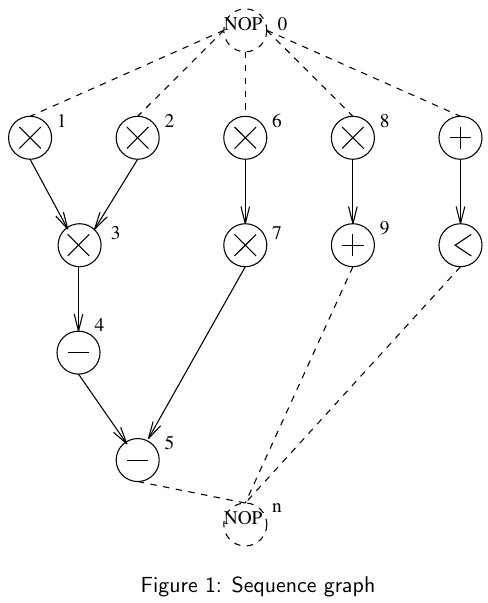
\includegraphics[height=0.6\paperheight]{./figures/task1_sequence_graph.png}
    \end{figure}
  \end{tasknoinc}
  \begin{tasknoinc}
    \begin{itemize}
      \item all operations are handled by the same resource type with a yet unspecified number of instances
      \item all operations have same execution time
    \end{itemize}
  \end{tasknoinc}
  \framebreak
  \begin{requirementsnoinc}
    \begin{figure}
      \centering
      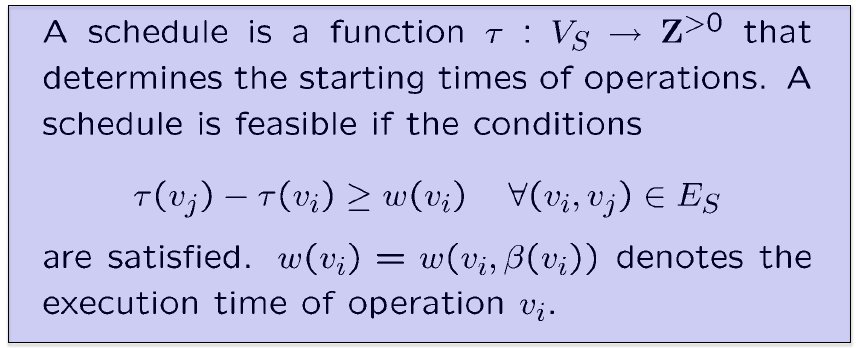
\includegraphics[height=0.4\paperheight]{./figures/task1_scheduleable.png}
    \end{figure}
  \end{requirementsnoinc}
  \begin{solutionnoinc}
    \begin{itemize}
      \item System of inequations:
        \[
          \begin{aligned}
            & \tau\left(v_3\right)\ge\tau\left(v_1\right)+1 \\
            & \tau\left(v_3\right)\ge\tau\left(v_2\right)+1 \\
            & \tau\left(v_4\right)\ge\tau\left(v_3\right)+1 \\
            & \tau\left(v_5\right)\ge\tau\left(v_4\right)+1 \\
            & \tau\left(v_5\right)\ge\tau\left(v_7\right)+1 \\
            & \tau\left(v_7\right)\ge\tau\left(v_6\right)+1 \\
            & \tau\left(v_9\right)\ge\tau\left(v_8\right)+1 \\
            & \tau\left(v_{11}\right)\ge\tau\left(v_{10}\right)+1 \\
          \end{aligned}
        \]
    \end{itemize}
  \end{solutionnoinc}
  \begin{solution}
        \[
          \begin{aligned}
            & \tau\left(v_1\right)\ge\tau\left(v_0\right) \\
            & \tau\left(v_2\right)\ge\tau\left(v_0\right) \\
            & \tau\left(v_6\right)\ge\tau\left(v_0\right) \\
            & \tau\left(v_8\right)\ge\tau\left(v_0\right) \\
            & \tau\left(v_{10}\right)\ge\tau\left(v_0\right) \\
          \end{aligned}
        \]
        \[
          \begin{aligned}
            & \tau\left(v_n\right)\ge\tau\left(v_5\right)+1 \\
            & \tau\left(v_n\right)\ge\tau\left(v_9\right)+1 \\
            & \tau\left(v_n\right)\ge\tau\left(v_{11}\right)+1 \\
          \end{aligned}
        \]
  \end{solution}
  \begin{requirementsnoinc}
    \begin{figure}
      \centering
      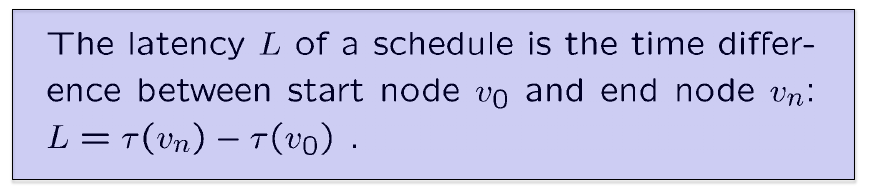
\includegraphics[height=0.2\paperheight]{./figures/task1_latency.png}
    \end{figure}
  \end{requirementsnoinc}
  \begin{solution}
    \begin{itemize}
      \item Initial condition:
        \[
        \tau\left(v_0\right)=0
        \]
      \item Objective function:
        \[
        \min \tau\left(v_n\right)-\tau\left(v_0\right)
        \]
    \end{itemize}
  \end{solution}
  \framebreak
  \begin{solutionnoinc}
    \begin{itemize}
      \item Minimum latency and valid starting times:
        \begin{itemize}
          \item One resource: $L_{\min }=11$
          \item Unlimited resources: $L_{\min }=4$
        \end{itemize}
    \end{itemize}
  \end{solutionnoinc}
  \begin{solutionnoinc}
    \begin{itemize}
        \item 1 resource: e.g.:
        \[
          \begin{gathered}
          \tau\left(v_1\right)=0 ; \tau\left(v_2\right)=1 ; \tau\left(v_3\right)=2 ; \tau\left(v_4\right)=3 ; \tau\left(v_6\right)=4 \\
          \tau\left(v_7\right)=5 ; \tau\left(v_5\right)=6 ; \tau\left(v_8\right)=7 ; \tau\left(v_9\right)=8 ; \tau\left(v_{10}\right)=9 \\
          \tau\left(v_{11}\right)=10 ; \tau\left(v_n\right)=L=11
          \end{gathered}
        \]
    \end{itemize}
  \end{solutionnoinc}
  \begin{solutionnoinc}
    \begin{itemize}
      \item Umlimited resources: e.g.
    \end{itemize}
    \begin{figure}
      \centering
      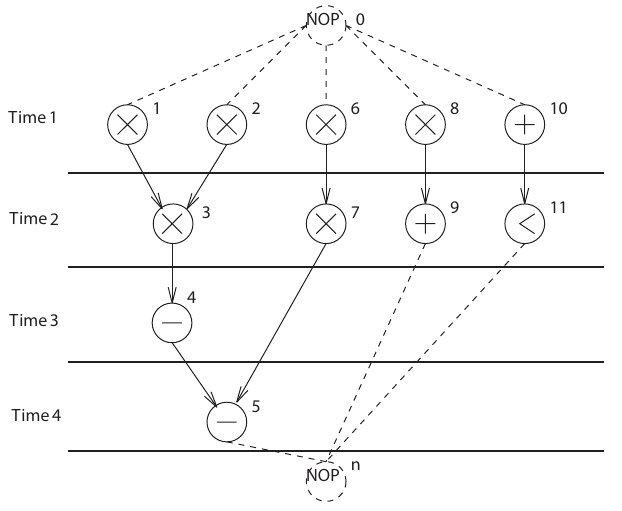
\includegraphics[height=0.5\paperheight]{./figures/task1_starting_times.png}
    \end{figure}
  \end{solutionnoinc}
\end{frame}
